
Теперь посмотрим на поведение характеристик в зависимости от параметров построения графов, при фиксированных распределениях
\begin{equation*}
    \text{Weibull}(\ \frac{1}{2}, \frac{1}{\sqrt{10}}) \qquad\qquad \Gamma(\ \frac{1}{2}, \frac{1}{\sqrt2})
\end{equation*}

\hspace*{-1cm}
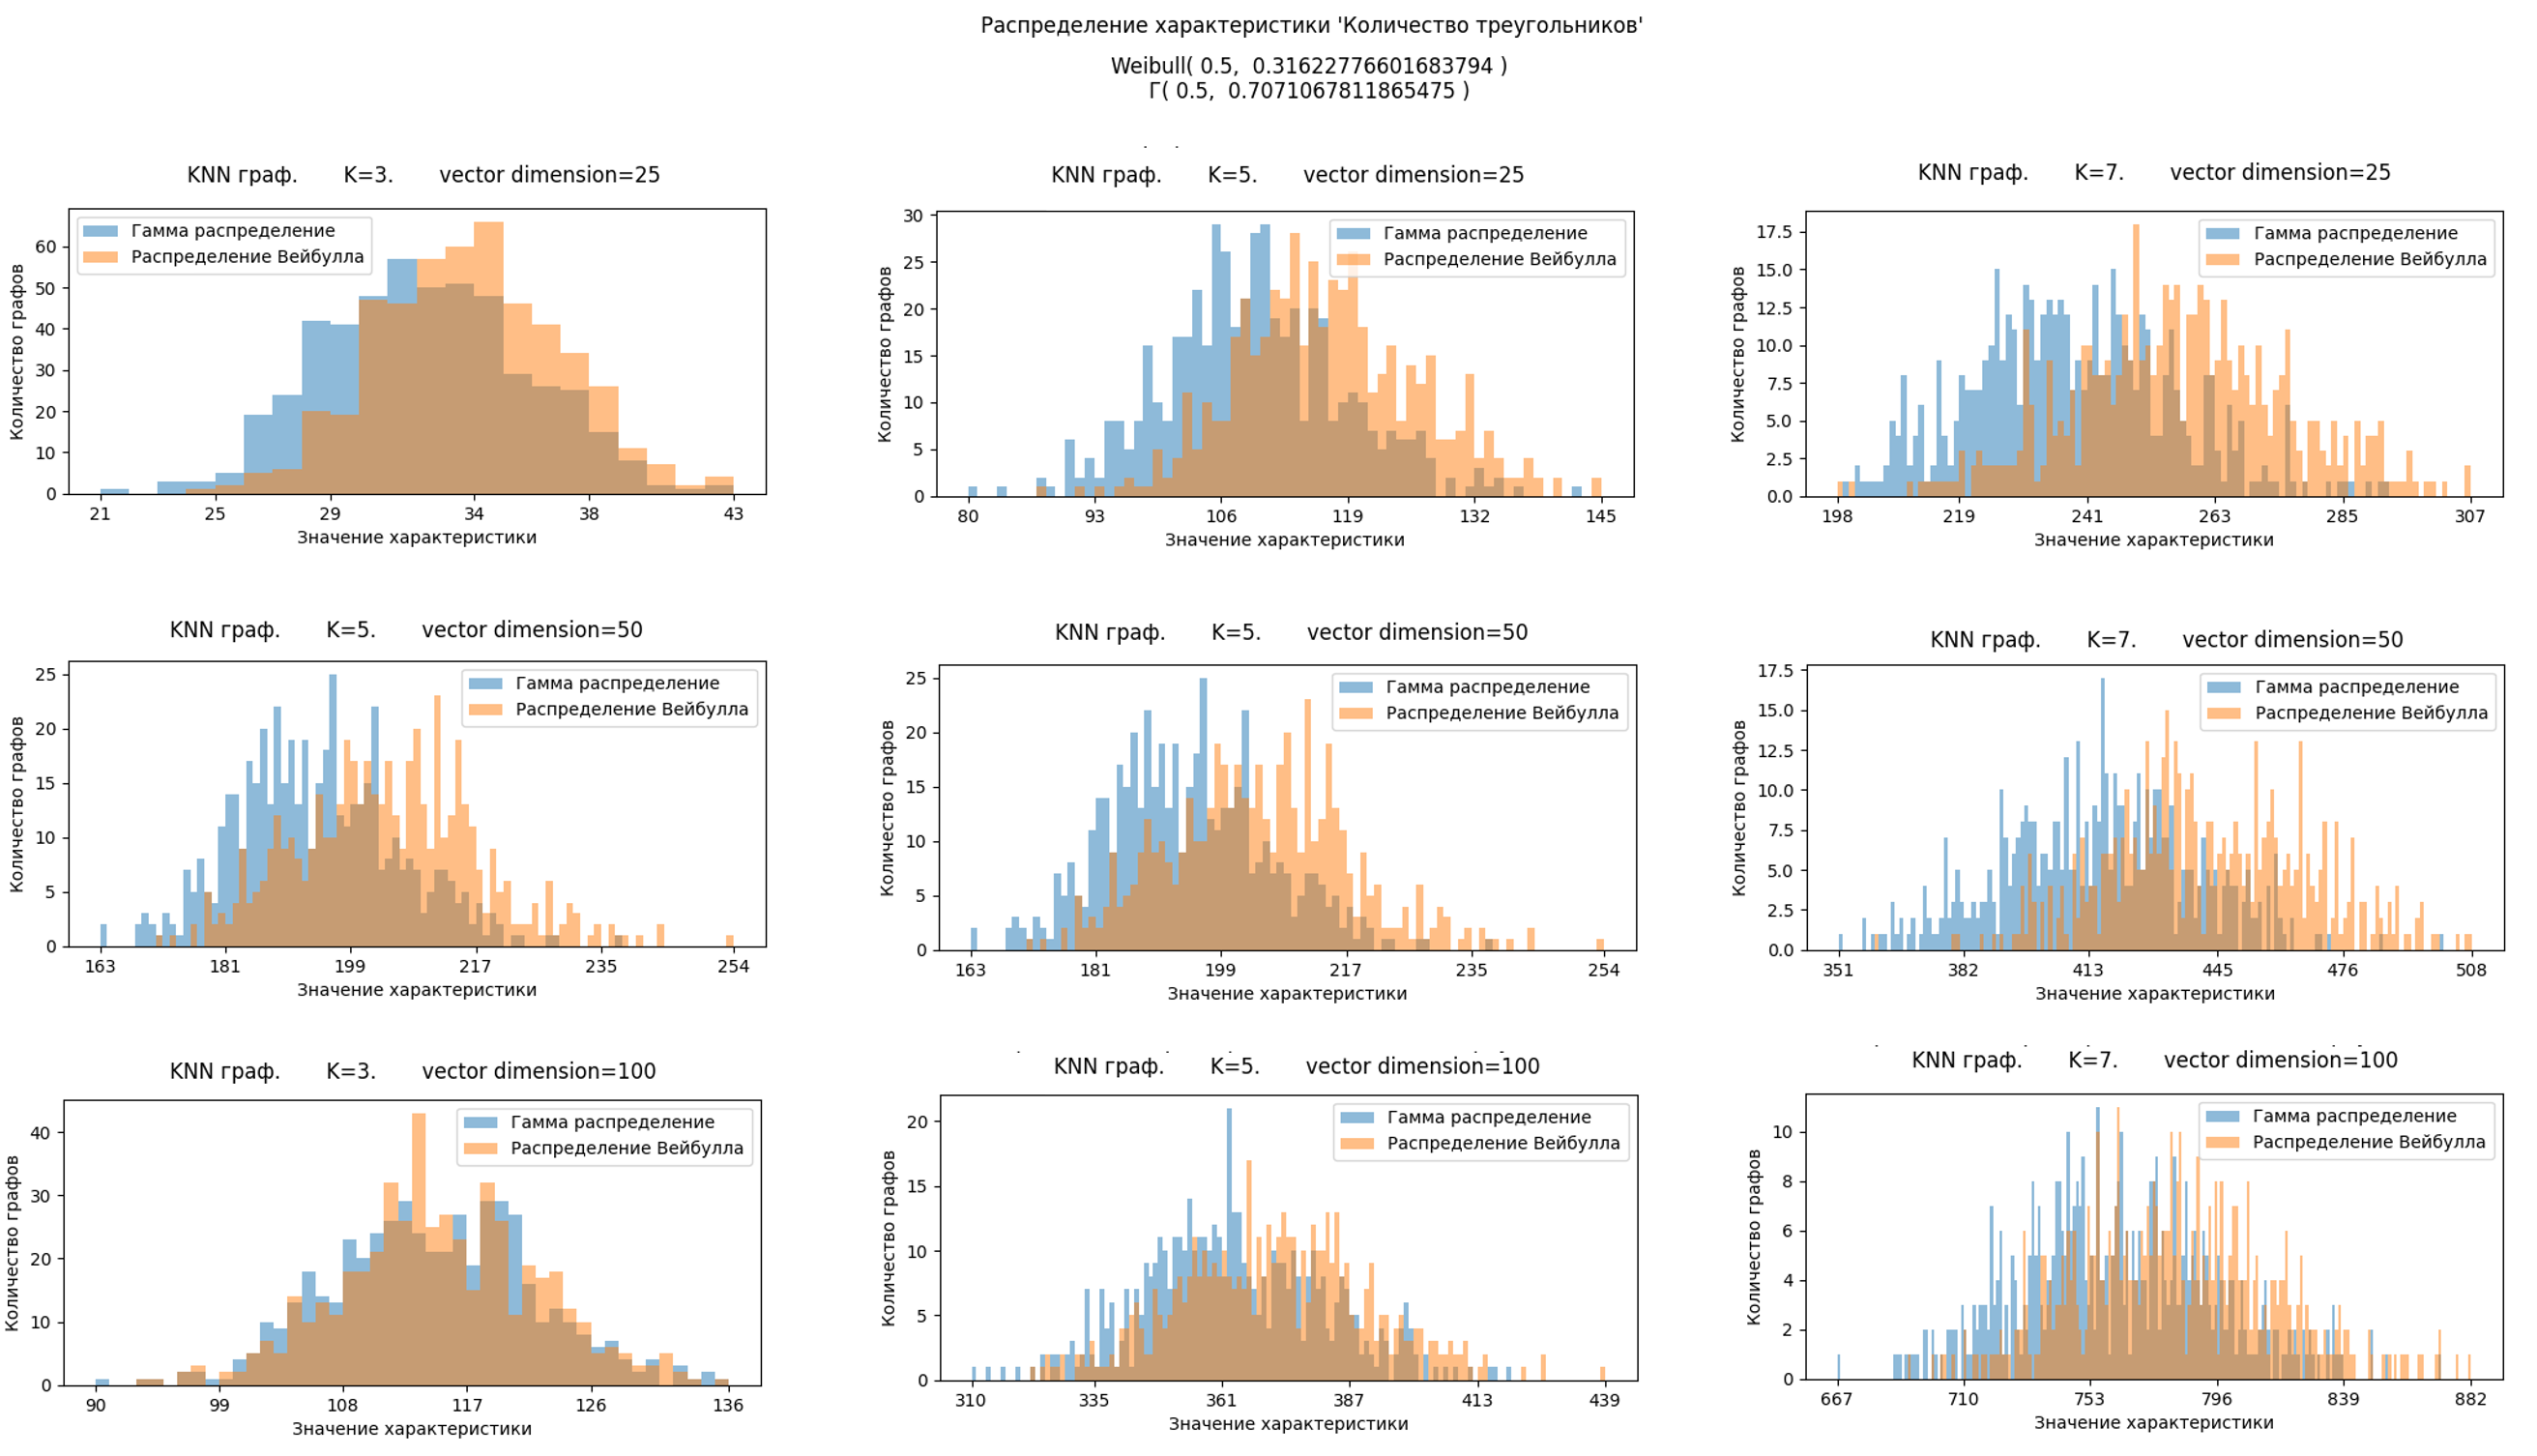
\includegraphics[width=1\textwidth]{Part-I_student-2/point 2_histogram_KNN.png}\\ 

\textbf{Вывод:} при большом размере выборки, количество треугольников выглядит как не самая удачная характеристика для классификации, однако, при относительно небольшой выборке ($\leq 50$), эта характеристика может оказаться неплохим второстепенным признаком.\\ 

\hspace*{-1cm}
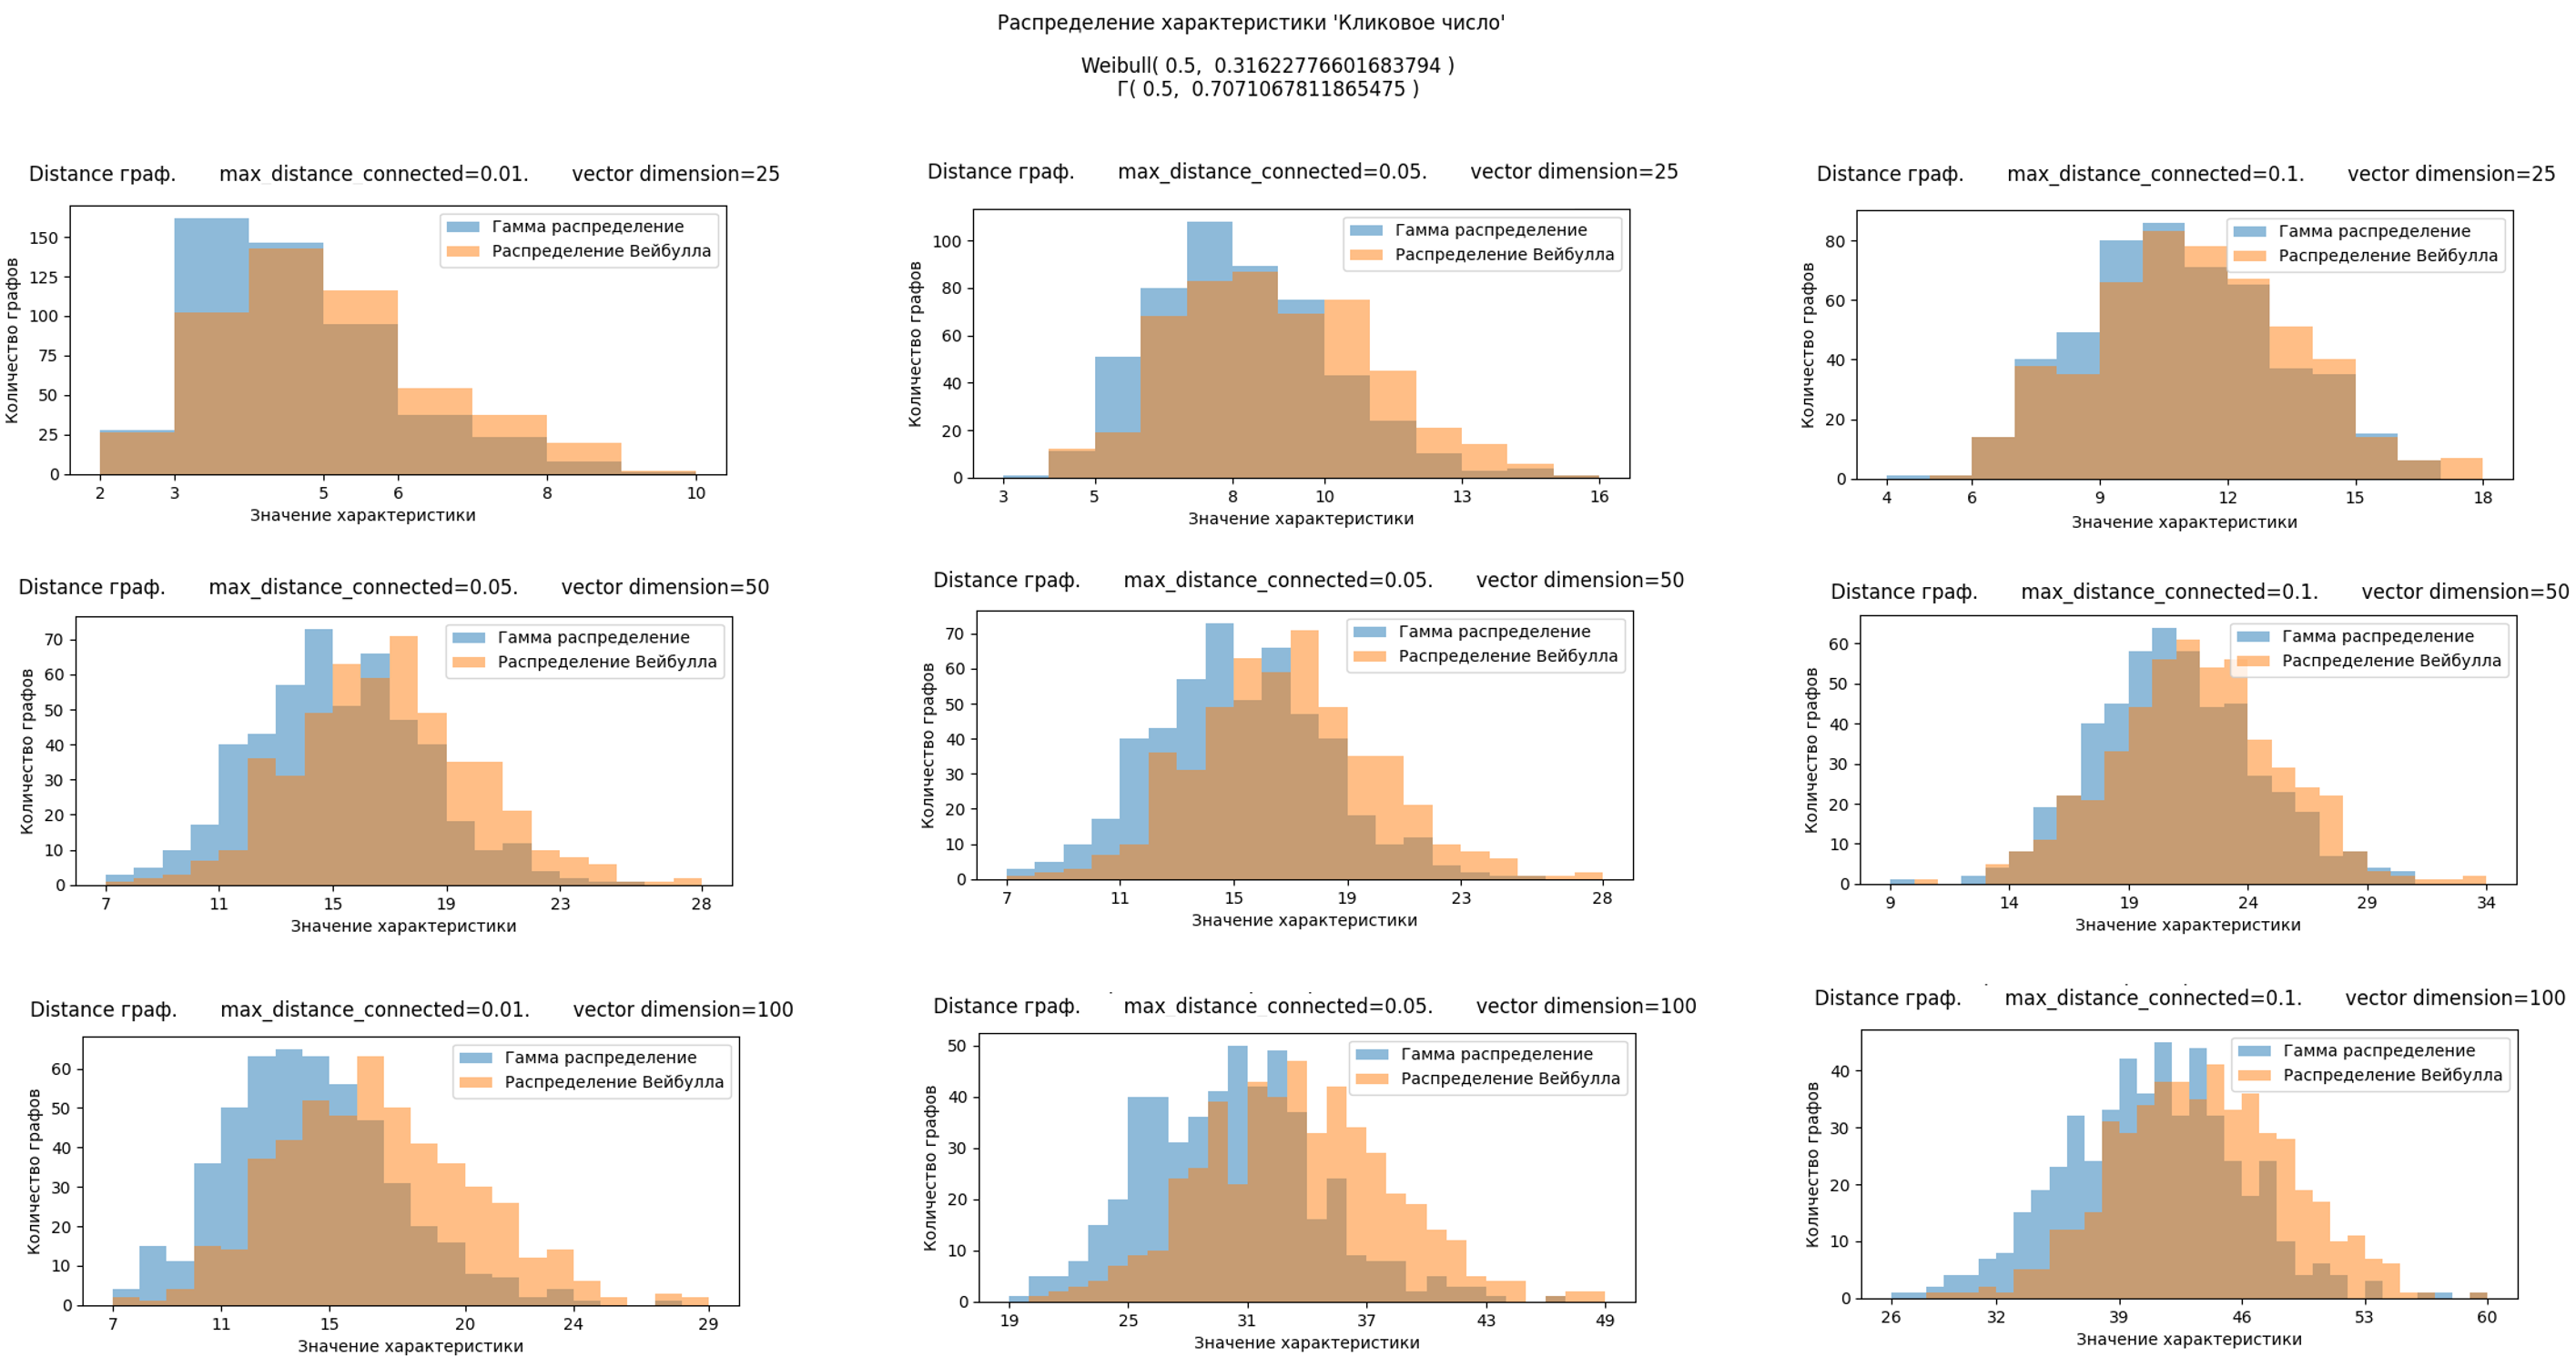
\includegraphics[width=1\textwidth]{Part-I_student-2/point 2_histogram_Dist.png}\\ 

\textbf{Вывод:} кликовое число, с точки зрения задачи классификации, для данных распределений является посредственным признаком, независимо от размера выборки и расстояния связи. Убедиться в этом  еще раз мы сможем в \textbf{Part-II}. 